% !TeX encoding = UTF-8
% !TeX spellcheck = ru_RU
\section{Вычисление максимальной дальности}
\textbf{Кишкун. Задание 1}
В сетях первого поколения дальность передачи была обусловлена только
тем, что необходимой была прямая видимость между абонентом
и базовой станцией.
\subsection{Постановка задачи}
Как вычислить максимальное расстояние между абонентом и базовой станцией в зависимости от высоты, на которой они расположены? Геометрическое представление задачи изображено на рисунке \ref{fig:img8}.

\begin{figure}[H]
	\centering
	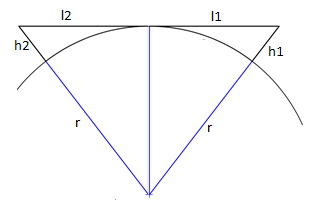
\includegraphics[width=0.5\textwidth]{img/kich_bur/image8.png}
	\caption{Геометрическое представление решаемой задачи}
	\label{fig:img8}
\end{figure}

$ h_1 $ --- высота антенны Базовой станции над поверхностью Земли 

$ h_2 $ --- высота антенны абонента над поверхностью Земли 

Земля --- идеальная сфера с радиусом $r = 6371$ км.

Максимальное расстояние между передатчиком и приемником будет тогда, когда прямая, соединяющая эти точки будет являться касательной к окружности. 

Предполагается, что частотный диапазон, мощность передатчика и чувствительность
приемника таковы, что если между передатчиком и приемником имеется
прямая видимость, то связь возможна вне зависимости от длины отрезка
между передатчиком и приемником. При относительно низких частотах
возможна передача за пределы прямой видимости. 

\subsection{Расчет физического расстояния}

Рассмотрим рисунок \ref{fig:img8}. По теореме Пифагора найдем длины $ l_1 $ и $ l_2 $: 

\[
(r+h_{1})^2=l_1^{2}+r_2
\]

\[
(r+h_{2})2=l_2^{2}+r_2
\]

\[
l1=\sqrt{h_{1}\left(h_{1}+2r\right)}
\]

\[
l2=\sqrt{h_{2}\left(h_{2}+2r\right)}
\]

Искомое расстояние: 

\[
L=\sqrt{h_{1}\left(h_{1}+2r\right)}+\sqrt{h_{2}\left(h_{2}+2r\right)}
\]

Расчет расстояния по поверхности: 

\[
\alpha_{1}=arctg(l_{1}/r)
\]

\[
\alpha_{2}=arctg(l_{2}/r)
\]

\[
C=(2*\pi*r*(\alpha1+\alpha2))/360
\]

\subsection{Доказательство оптимальности решения}
На рисунке \ref{fig:img9} показан случай, когда передатчик и приемник находятся дальше допустимого расстояния. Передаваемый сигнал будет гаситься землей.

\begin{figure}[H]
\centering{}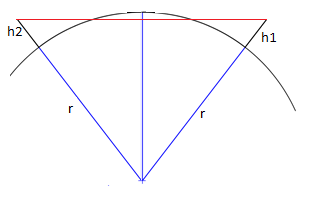
\includegraphics[width=3.27in,height=2.15in]{img/kich_bur/image9.png}
\caption{Превышение допустимого расстояния}
\label{fig:img9}
\end{figure}

Рассмотрим вариант, изображенный на рисунке \ref{fig:img10}. В этом случае передатчик и приемник находятся ближе допустимого расстояния. Сигнал будет проходить над поверхностью земли и расстояние между передатчиком и приемником не будет максимальным. 

\begin{figure}[H]
\centering{}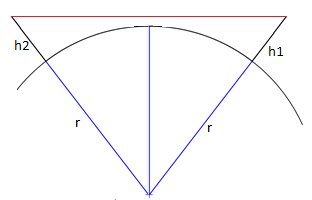
\includegraphics[width=3.25in,height=2.08in]{img/kich_bur/image10.png}
\caption{Уменьшение расстояния}
\label{fig:img10}
\end{figure}

Таким образом, для нахождения максимального расстояния между передатчиком и приемником в зависимости от их высот, когда единственным фактором обеспечения связи является прямая видимость, обусловленная кривизной
земли, оптимальным является решение, когда прямая, соединяющая эти точки будет являться касательной к окружности.

Для проверки формулы была создана программа на Matlab [\ref{code:code7}]:
\lstinputlisting[language=Matlab, label=code:code7, captionpos=b, caption=Расчет максимального расстояния]{src/7.m}

Результаты вычислений представлены в таблице \ref{tab:table1}. 
\begin{table}
	\centering
	\resizebox{\textwidth}{!}{%
	\begin{tabular}{|p{6cm}|p{4cm}|p{4cm}|p{6cm}|}\hline
		Максимальное расстояние между передатчиком и приемником (C, км)&Высота абонента ($ h1 $, м)&Высота базовой станции $ (h2 $, м)&Сравнительная высота\\ \hline
		5.0977&1.6 & 1.75&Рост человека\\ \hline 
		12.4775&1.6&25&9-этажный дом\\ \hline
		16.3774&1.6&50&Колесо обозрения\\ \hline 
		26.3877&1.6&150&Воздушный шар\\ \hline 
		80.9754&1.6&2000&Гора\\ \hline 
		132.7091&1.6&10000&Самолет\\ \hline
		175.1684&1.6&350000&Космический корабль\\ \hline
		260.4347&10000&10000&Передатчик и приемник на 
		высоте полета самолета\\ \hline
		15.0337&1.75&40&Стандарт 1G\\ \hline
		40.0&25&250&Максимальное расстояние для сетей первого поколения\\ \hline
	\end{tabular}}
	\caption{Результаты вычислений}
	\label{tab:table1}
\end{table}
\newpage